\subsection*{Hypothesis 2}
This hypothesis investigates whether reviews containing a higher number of positive sentiment words
tend to receive more helpfulness ratings.\\
Before testing this hypothesis, it is necessary to define what is meant by "positive sentiment words".
To do so, a Multinomial Naive Bayes classifier was trained on the dataset,
with adjustments made to consider words with a score greater than 3 as positive reviews and those
with a score less than 3 as negative reviews. Positive sentiment words were identified by calculating
the difference in word weights between the positive and negative classes.
Among these words, those with weights greater than 0 were deemed positive sentiment words.
Only the top 800 words with the highest weights were retained for further analysis.\\
Subsequently, the frequency of these positive sentiment words was computed for each review.
The correlation between the frequency of these words and review helpfulness was then calculated.
Given that the features do not follow a normal distribution, the Spearman correlation coefficient was used.\\
The result yielded a correlation coefficient of 0.318 with a p-value < 0.05, indicating statistical significance in general.
However, the correlation value becomes negative for a number of words higher than 100, as shown in Figure \ref{fig:corr_pos_words}.

\begin{figure}[H]
    \centering
    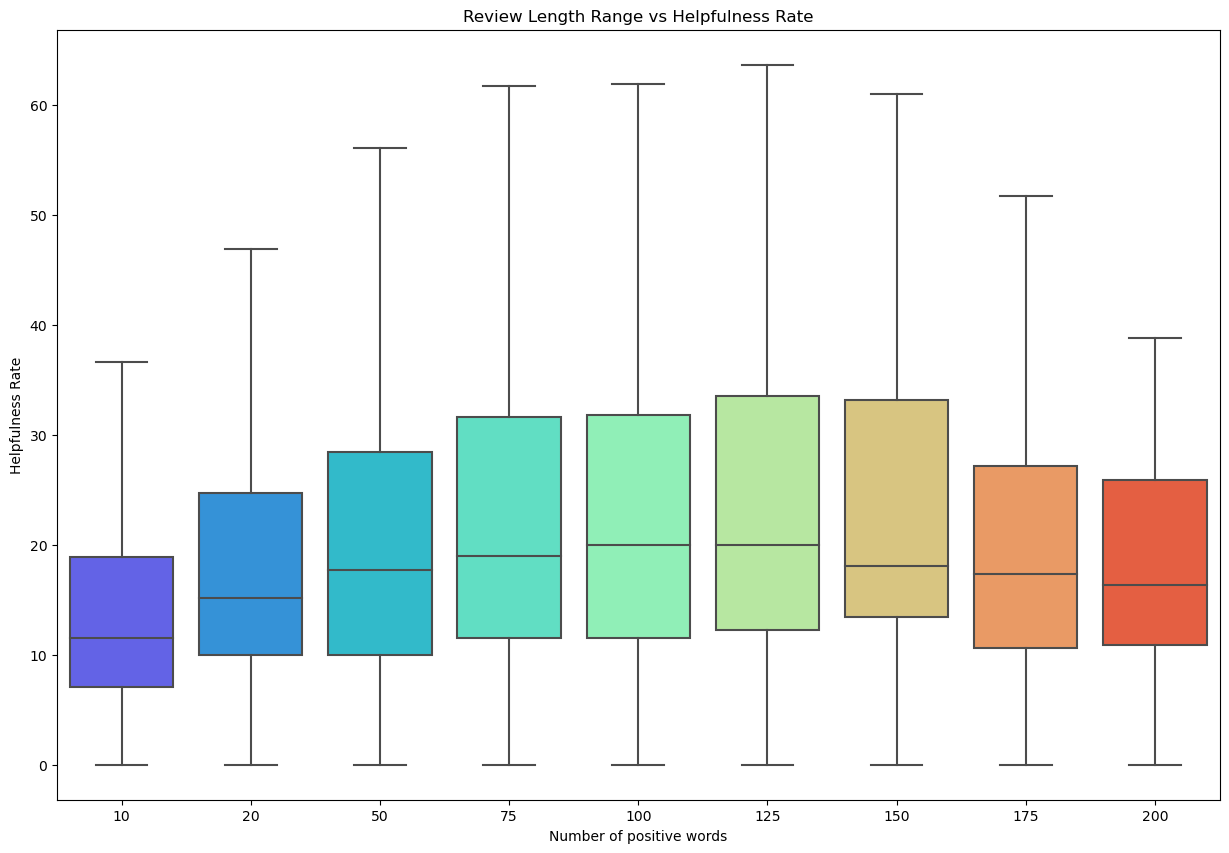
\includegraphics[width=0.4\textwidth]{./figures/h2.png}
    \caption{Correlation between the frequency of positive sentiment words and review helpfulness}
    \label{fig:corr_pos_words}
\end{figure}
